% Diagrama del pipeline experimental (M1 de la guia). Hecho a mano en TikZ,
% sin IA de imagenes (guia metodologica 4.1): cajas rectangulares, trazo fino,
% grises, sans-serif (guias de AICE: Helvetica/Arial). Se compila aparte y se
% incluye como un unico PDF, porque Springer pide un archivo por figura.
%   pdflatex fig_pipeline.tex
\documentclass[tikz,border=2pt]{standalone}
\usepackage{helvet}% sin escalar: \footnotesize = 8 pt, el minimo de AICE
\renewcommand{\familydefault}{\sfdefault}
\usetikzlibrary{positioning,arrows.meta,fit}
\begin{document}
% Sin palabras partidas con guion dentro de las cajas estrechas.
\hyphenpenalty=10000 \exhyphenpenalty=10000
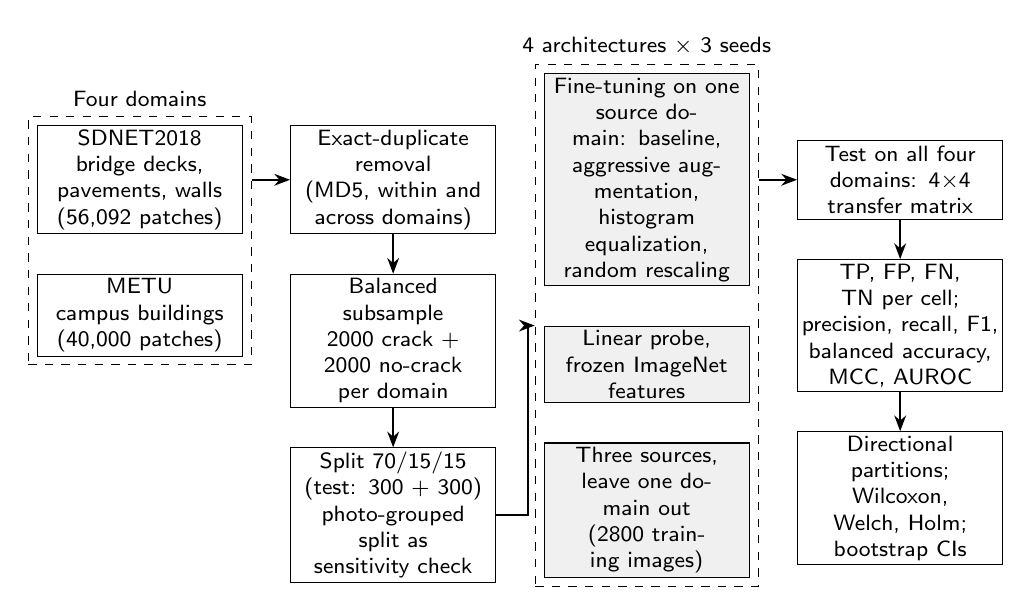
\begin{tikzpicture}[
  font=\footnotesize,
  caja/.style={draw, rectangle, align=center, minimum height=10mm, text width=25mm, inner sep=1.5pt},
  grupo/.style={draw, rectangle, fill=black!6, align=center, text width=25mm, inner sep=1.5pt},
  flecha/.style={-{Stealth[length=2mm]}, semithick},
  node distance=5mm and 6mm
]
% Columna 1: datos
\node[caja] (sd) {SDNET2018\\bridge decks, pavements, walls\\(56,092 patches)};
\node[caja, below=of sd] (metu) {METU\\campus buildings\\(40,000 patches)};
\node[draw, dashed, inner sep=3pt, fit=(sd)(metu), label={[font=\footnotesize]above:Four domains}] (datos) {};

% Columna 2: preparacion
\node[caja, right=6mm of sd] (dedup) {Exact-duplicate removal\\(MD5, within and\\across domains)};
\node[caja, below=of dedup] (sub) {Balanced subsample\\2000 crack + 2000 no-crack\\per domain};
\node[caja, below=of sub] (split) {Split 70/15/15\\(test: 300 + 300)\\photo-grouped split as\\sensitivity check};

% Columna 3: regimenes de entrenamiento
\node[grupo, right=6mm of dedup] (ft) {Fine-tuning on one\\source domain: baseline,\\aggressive augmentation,\\histogram equalization,\\random rescaling};
\node[grupo, below=of ft] (lp) {Linear probe,\\frozen ImageNet\\features};
\node[grupo, below=of lp] (loo) {Three sources,\\leave one domain out\\(2800 training images)};
\node[draw, dashed, inner sep=3pt, fit=(ft)(lp)(loo), label={[font=\footnotesize, align=center]above:4 architectures $\times$ 3 seeds}] (reg) {};

% Columna 4: evaluacion y analisis
\node[caja, right=6mm of ft] (eval) {Test on all four\\domains: 4$\times$4\\transfer matrix};
\node[caja, below=of eval] (metr) {TP, FP, FN, TN per cell;\\precision, recall, F1,\\balanced accuracy,\\MCC, AUROC};
\node[caja, below=of metr] (stat) {Directional partitions;\\Wilcoxon, Welch, Holm;\\bootstrap CIs};

\draw[flecha] (datos.east |- dedup.west) -- (dedup.west);
\draw[flecha] (dedup) -- (sub);
\draw[flecha] (sub) -- (split);
\draw[flecha] (split.east) -- ++(4mm,0) |- (reg.west);
\draw[flecha] (reg.east |- eval.west) -- (eval.west);
\draw[flecha] (eval) -- (metr);
\draw[flecha] (metr) -- (stat);
\end{tikzpicture}
\end{document}
